\documentclass{UoYCSproject}
\usepackage{color,soul}
\usepackage{graphicx}
\usepackage{amsmath}
\usepackage{textgreek}
\usepackage{amssymb}

\addbibresource{refs.bib}

\author{Patrick Buhagiar}
\title{The Impact of Macroeconomic Parameters on Forecasting Financial Markets}
\date{2018-July-06}
\supervisor{Dimitar Kazakov}
\MIP
\wordcount{8832}

\includes{Appendices \ref{cha:usefulpackages}, \ref{cha:gotchas} and
  \ref{cha:deptfac}}

\excludes{\autoref{cha:quoteex}}

\abstract{ 
    Financial forecasting is a common area in machine learning, however a gap in literature was identified with respect to the influence of macroeconomic variables in predicting financial markets. This study attempts to use ensemble methods to predict the direction of the FTSE market in relation to other financial markets and macroeconomic variables in the UK. This study adopts a two-stage process. The first stage consists of creating several ANN models for different time periods that predict the stock market based on the closing prices of other markets. The second stage consists of feeding the results from the first stage and macroeconomic data into another ANN. \hl{TODO add result summary as last sentence}
}

\dedication{To all students everywhere}

\acknowledgements{To my cactus, that I forget to water}
\bibliography{refs}
\begin{document}

\maketitle

\listoffigures
\listoftables

\label{sec:start}
\thispagestyle{empty}\cleardoublepage

\chapter{Introduction}
\label{cha:literaturereview}

\chapter{Background}
\label{cha:background}

\section{Macro and Micro Economics}
According to Adam Smith, the first modern economist, the economy is a mix of micro and macro economics where every entity has individual interest towards gain, such that this gain is also linked to the overall benefit of the market as a whole \cite{smith1950inquiry}. Macroeconomics is the study of the behaviour, performance and trends of an economy as a whole. Macro-economists evaluate a variety of economy-wide phenomena such as inflation, gross domestic product (GDP) and unemployment. To keep the economy in check, governments look at these factors to aid in economic policy decision making. Microeconomics on the other hand is the study of how individuals make economic decisions and their effect on the economy. These individuals are classified into consumers, producers and resource owners \cite{dwivedi2002microeconomics}. These individuals interact with the supply and demand for resources while using indications such as interest rates and money as a pricing mechanism for coordination. 

Despite being split into two different studies, macroeconomics and microeconomics are deeply interlinked with each other since they contain overlapping issues. They can be considered as opposite approaches, where macroeconomics take a top-down approach and microeconomics a bottom-up approach to analysing an economy. As an example of how these two studies complement each other, it is evident that a stock market's long-run performance is heavily coupled with the economy's performance \cite{davis2008macroeconomic}. This coupled relationship can be seen in Figure \ref{fig:gdpvssp500} which shows a normalised plot for the U.S. GDP and the S\&P 500 index. In this case, it comes to no surprise that investment analysts focus on economic performance expectations to determine the future prospects of stock markets.

\begin{figure}[h]
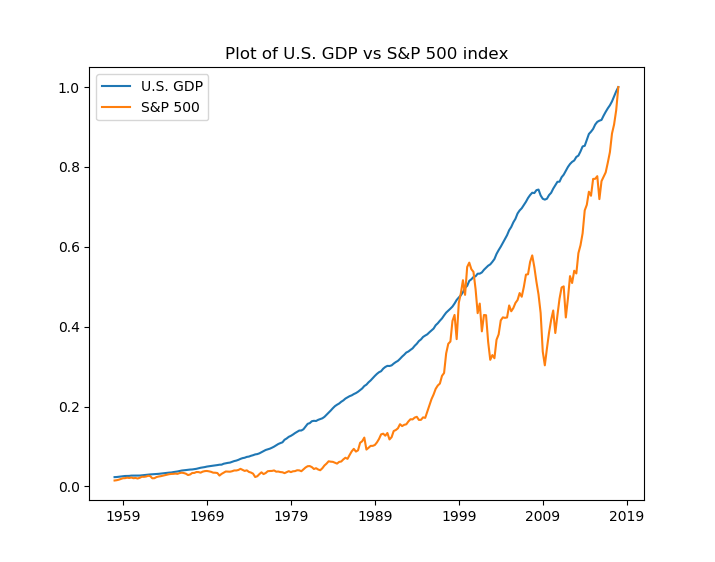
\includegraphics[width=10cm]{GDPvsSP500}
\centering
\caption{Normalised quarterly data from 1958 to 2018 for U.S. GDP and S\&P 500 index. Sources: Standard \& Poor's, U.S. Census Bureau} 
\label{fig:gdpvssp500}
\end{figure}

\subsection{Inflation}
Inflation is the rate at which the general level of prices for goods and services is rising \cite{inflation}. As a result of inflation, the purchasing power of a currency decreases. If the price of milk costs \pounds 1 this year, then with an inflation rate of 2\% it will cost \pounds 1.02 the following year. Deflation is the opposite of inflation, where the general level of prices decreases. Central banks define this inflation rate and try to limit inflation, while avoiding deflation, so as to keep the economy running smoothly. While over inflation should be avoided, deflation is much more catastrophic and has helped cause the worst economic meltdowns in U.S. history \cite{fleckenstein2013deflation}. If there is deflation, people refrain from consuming goods because they know that they will be cheaper in the future. This will reduce the demand for goods drastically which will translate into a reduction in corporate profits, lower wages, a reduction in work force and thus a weaker economy. For an economy to be functioning well, both the consumers and producers must be willing to consume and produce. 

\subsection{Balance of Trade}
The balance of trade is the difference between the value of a country's imports and exports during a certain period \cite{balanceoftrade}. Economists refer to the balance of trade to measure the relative strength of a country's economy. The balance of trade can be calculated with the following simple formula:

\begin{equation}
    Balance Of Trade = Imports - Exports
\end{equation}

When a country imports more than it exports, it would have a trade deficit, otherwise if it exports more than it imports it would have a trade surplus. A country that has a trade deficit borrows money. This could lead to the value of the country's currency to fall, which will result in consumers paying more for foreign imports \cite{2003economics}. Alternatively a country that has a trade surplus lends money to deficit countries. As of 2016, the country with the highest trade surplus is China with a surplus of \$510 Billion \cite{tradesurplus}.   

\subsection{GDP}
Historically, GDP (gross domestic product) is one of the most important variables when it comes to measuring the health of an economy. A country's GDP is the total value of all final goods and services produced in the economy \cite{2003economics}. GDP helps define the size of an economy. The bigger the GDP, the more goods are being produced, therefore the healthier the economy is.  There are many factors that effect the GDP such as life expectancy, higher initial schooling, lower inflation and lower fertility \cite{barro1996determinants}. 

\subsection{Unemployment Rate}

The unemployment rate is the percentage of the labour force that is jobless \cite{unemployment}. In a weak economy, jobs tend to be scarce, hence the unemployment rate is expected to rise. Alternatively, a healthy economy is more likely to have more jobs available, thus the unemployment rate will decrease. This means that unemployment rate is another factor that highly affects a country's GDP \cite{bean1993unemployment}. A low unemployment rate means that more people are employed and getting paid, which brings in more money into the economy, ergo increase GDP.  

\subsection{Interest Rate}
An interest rate is a percentage of the amount that one pays when borrowing or gets paid when saving money \cite{interestrate}. If \pounds 1000 is placed into a savings account with a 1\% interest rate, there will be \pounds 1010 the following year.  The bank rate is the most important interest rate in an economy and is set by the central bank. The bank rate is the rate of interest payed on reserve balances held by commercial banks. Increasing the bank rate makes borrowing more expensive which means people will spend less in order to pay off their debts or benefit more from saving. In this scenario, inflation will decrease. Ultimately, interest rates can be considered as a tool for monetary policy that can be used to contain inflation within an expected range \cite{christiano1999monetary}. 

\section{Financial Markets}
A financial market is a marketplace for buying and selling securities such as stocks, bonds and currencies \cite{financialmarket}. Trading occurs on what is called an exchange. In the case of stocks, this is called a stock exchange and can either be in a physical location (like NYSE) or an electronic system (like NASDAQ). Any company that is traded on an exchange is referred to as a listed company, otherwise securities that are not listed are sold Over-The-Counter (OTC). Companies that trade shares OTC are typically smaller and riskier companies that did not meet the requirements to be listed on the stock exchange \cite{stockexchange}. As of June 2017, the stock exchange with the highest market capitalisation is the New York Stock Exchange (NYSE) with \$21 trillion \cite{nyse}. 

\subsection{Stock Market Index}
Another way to measure the value of a stock market, other than the total market capitalisation, is to use what is called a stock market index. A stock market index is computed from the prices or market capitalisation of a few selected stocks, typically from the largest and most influential companies in that market. The Dow Jones Industrial Average (DJIA) is one of the oldest, most well-known stock market index in the world, which takes the stocks prices of 30 companies in the United States across different industries, such as Apple, American Express, Coca-Cola and ExxonMobil. Experts however feel that the DJIA is \textit{"no longer a great reflection of the market anymore [since] it only covers 30 stocks [and] puts too much emphasis on the price rather than a market's capitalization"} \cite{dowproblem}. For the United States, a better alternative is the S\&P 500, which is much more diverse than DJIA because it includes 500 companies and uses a market capitalisation-weighted index. The main goal of these stock market indices is to represent a broad economy. Table \ref{tab:indices} lists a few of the most common stock indexes, along with their region and the number of companies they represent. 

\begin{table}[h]
    \centering
    \begin{tabular}{|c|c|c|c|} \hline
        \textbf{Index} & \textbf{Trading Symbol} & \textbf{Region} & \textbf{\# of Companies} \\ \hline
        DOW 30 & DJI & U.S.A & 30 \\
        S\&P 500 & GSPC & U.S.A & 500 \\
        NASDAQ 100 & NDX & U.S.A & 100 \\
        FTSE 100 & FTSE & United Kingdom & 100 \\
        DAX & GDAXI & Germany & 30 \\
        CAC 40 & FCHI & France & 40 \\
        EURO STOXX 50 & STOXX & Eurozone & 50 \\
        NIKKEI 225 & N225 & Japan & 225 \\
        HANG SENG & HSI & Hong Kong & 50 \\
        \hline
    \end{tabular}
    \caption{Table of Popular Stock Market Indices}
    \label{tab:indices}
\end{table}

\subsection{Market Hypotheses}
\subsubsection{Efficient Market Hypothesis}
The Efficient Market Hyptothesis (EMH) was introduced by Fama in 1970  \cite{malkiel1970efficient} and is frequently cited in the field of finance and economics as it is a ubiquitous theory in modern finance. It states that a market is said to be efficient if the stock price of a company at any given time truly reflects the value of that company. This means that there is no point in studying past stock prices in search for patterns to predict future prices. While many academics refer to a large body of evidence in support of EMH, an equal amount of evidence also contradicts EMH. Jensen's \cite{jensen1978some} paper finds that as better data is becoming available, such as daily stock prices, the more inconsistencies are beginning to be found with EMH. It concludes that there are flaws with EMH and over time we will better understand these flaws and thus a better understanding of the markets. Another paper by Malkiel \cite{malkiel2003efficient} points out that while evidence has proved EMH to be useful in the past, certain conditions have deemed EMH inefficient for the current modern economy. Nonetheless, economists have not yet reached a consensus about whether financial markets are indeed efficient \cite{lo2004adaptive}.  

\subsubsection{Adaptive Market Hypothesis}
AMH is an improved version of EMH by Andrew Lo \cite{lo2004adaptive}. He explains that emerging study has challenged EMH, arguing that markets are actually driven by fear and greed rather than being rational. AMH seeks to add behavioural alternatives to EMH by applying the principles of evolution to financial interactions where the market is seen as an evolving entity \cite{lo2004adaptive}. These evolutionary principles are competition, adaptation and natural selection. Lo further expands on AMH in another paper \cite{lo2005reconciling}
by delving into a neuroscience perspective. As summarised by Matthew Butler \cite{butler2012computational}, the primary components of the AMH are:

\begin{enumerate}
\item Individuals act on their own self interest.
\item Individuals make mistakes.
\item Individuals learn and adapt.
\item Competition drives adaption and innovation.
\item Natural selection shapes market ecology.
\item Evolution determines market dynamics.
\end{enumerate}

The first item on the list is also true for EMH and is described as the underlying driver of capital markets in Adam Smith's "\textit{The Wealth of Nations}" \cite{smith1957}. The rest of the list however is unique to AMH.

\subsection{Random Walk Hypothesis}
The random walk hypothesis is another financial theory that is consistent with EMH. It states that stock prices are random, and thus cannot be predicted. It was introduced in Burton Malkiel's book "\textit{A Random Walk Down Wall Street}" \cite{malkiel1973random}. Similar to EMH, it also suggests that there is no point in exploiting patterns in historical data to gain profits.  

\subsection{Chaos Theory}
Chaos theory is a mathematical concept that deals with nonlinear models, therefore anything that is effectively impossible to predict or control, such as weather, brain states or, in our case, stock markets. It is quite controversial and complicated. In chaos theory, price changes can be determined through mathematical equations predicting factors such as a trader's own personal motives, volume changes, acceleration of the changes, and the momentum behind the changes \cite{chaostheory}.

\section{Analysis Techniques}
\subsection{Technical Analysis}
Technical analysis assumes that history tends to repeat itself, thus analysing past patterns can be used for predictive purposes \cite{levy1966conceptual}. For financial markets, this means looking at past stock prices for predictions rather than its components. There are three major assumptions:
\begin{enumerate}
    \item The stock price is reflective of the entire company's influential factors.
    \item Stock price movements follow trends.
    \item History repeats itself in terms of price movements.
\end{enumerate}

\subsection{Fundamental Analysis}
Fundamental analysis takes a wider approach than technical analysis by studying the past and present market data, as well as economic-level, industry-level and company-level indicators such as earnings, risk, growth and competitive position. Papers such as that of Lev and Thiagarajan \cite{lev1993fundamental} attempt to identify which fundamentals or financial variables, over a certain period of time, where suitable for performing financial forecasting. These fundamentals can either be quantitative or qualitative. Quantitative fundamentals are numeric values such as revenue and profit, while qualitative fundamentals are those that are based on the character or quality of a variable, such as brand recognition and competitive position. 

Unlike technical analysis, fundamental analysis assumes that the stock market is not fully representative of the actual value of the stock. fundamentalists however do believe that the market will reflect these fundamentals in the long run, thus encouraging investors to find opportunities to buy stocks at a reduced price by estimating the actual value of the stock. 

\subsection{Time series Analysis}
A time series is a collection of numerical data points collected at constant time in a form of a sequence. With time series analysis, we can obtain meaningful statistics and other characteristics of data, thus we can understand the data and build a model based on the given pattern. Extracting such models will allow us to forecast future values. 

Two key properties about time series are that they are time dependent, and that most time series have some form of seasonality trends. Seasonality trends mean that the time series consists of variations specific to a particular time frame. Due to these properties, forecasting time series requires the data to be stationary. A time series is said to be stationary if its neither the mean nor the autocovariances depend on the date \cite{hamilton1994time}. 

\subsubsection{Making a Series Stationary}
There are several methods for making a time series stationary, some of which can be combined together:
\begin{enumerate}
    \item \textbf{Transformation:} Trend can be reduced by transforming the data. this can be anything from calculating the log, square-root, cube root etc.  
    \item \textbf{Moving Average:} This method takes the average of \textit{k} consecutive values, depending on the frequency of the time series, for example 12 months, or 1 year. This is also called a \textit{rolling mean}. 
    \item \textbf{Differencing:} This technique involves subtracting each value with it's previous value.
    \item \textbf{Decomposition:} This approach consists of modelling trend and seasonality separately, and returning the remaining part, typically referred to as \textit{residual}. 
\end{enumerate}

\subsubsection{How to Test for Stationarity}
Statistical tests can be utilised to examine the stationary assumptions by decomposing the time series into three elements: trend, random walk, and stationary error. Two popular tests are Kwiatkowski-Phillips-Schmidt-Shin (KPSS) test and the Augmented Dickey-Fuller (ADF) test.

The ADF test was introduced in 1979 by David Dickey and Wayne Filler \cite{dickey1979distribution}. This test is used to determine whether a unit root, a stochastic feature that can cause problems in statistical inference, is present in an autoregressive model. 

The KPSS method proposes a test of the null hyphotesis that a series is stationary around a deterministic trend \cite{kwiatkowski1992testing}. While the ADF test's null hypothesis is the presence of a unit root, the null hypothesis for KPSS is the opposite. 

\printbibliography

\end{document}